%-------------------------------------------------------------------------------
\section{Introduction}
%-------------------------------------------------------------------------------

%-------------------------------------------------------------------------------
\section{Results}
%-------------------------------------------------------------------------------

\subsection{Coherence}

Spectral coherence is the Fourier analogue of linear correlation.
We computed the coherence between the \SIrange{31.3}{97.8}{Hz} range for pairs of depths.
Coherence between channels was computed using the Welch method using \SI{256}{\milli\second} windows with \SI{50}{\percent} overlap.

\begin{figure}
\centering 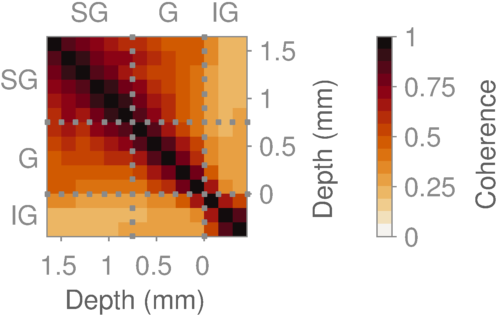
\includegraphics{coherence-avg_paper.png}
%
\caption{%
Coherence \SIrange{31.3}{97.8}{Hz}
}
\label{fig:lam_coher}
%
\end{figure}

The results show the same compartmentalisation as we observed for the information redundancy in the high frequency range.

Our results are in agreement with \citet[Figure 5B]{Maier2010}.

%-------------------------------------------------------------------------------
\section{Discussion}
%-------------------------------------------------------------------------------
